\section{Auswertung}
\subsection{Bestimmung der Strahlhöhe}
Zur weiteren Auswertung der aufgenommenen Daten ist es zunächst notwendig die Strahlhöhe zu berechnen. Hierzu werden die Messwerte des Detektorscans mit einer Gaußfunktion der Form
\begin{equation}
  f(x)=a\cdot \exp\left(-\frac{(x-\mu)^2}{2\sigma^2}\right)\,,
\end{equation}
gefittet und es wird die Halbwertsbreite bestimmt, welche die Strahlhöhe angibt.
\begin{figure}[h]
  \centering
  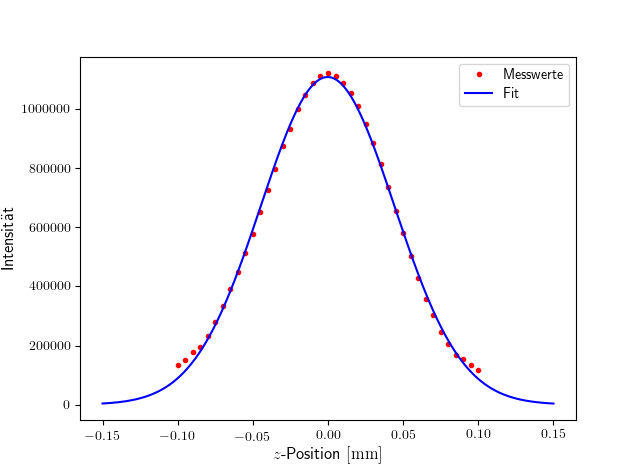
\includegraphics[width=\textwidth]{Bilder/fwhm.png}
  \caption{Messwerte des Detektorscans mit Fit.}
\end{figure}
Als Fitparameter ergeben sich
\begin{align}
a&=(1{,}109\pm0{,}005)\cdot10^6\nonumber\\
\mu&=(-0{,}00026\pm0{,}00024)\,\si{\mm}\nonumber\\
\sigma&=(0{,}0444\pm0{,}0003)\,\si{\mm}\,.
\end{align}
Die Strahlhöhe bestimmt sich zu
\begin{equation}
d_0=2\sqrt{2\ln2}\sigma=(0{,}1047\pm0{,}0006)\,\si{\mm}\,.
\end{equation}\\
\subsection{Berechnung des Geometriefaktors}
Zur Bestimmung der Parameter der Probe ist es zunächst notwendig den Geometriefaktor $G$
\begin{equation}
  G =
     \begin{cases}
       \frac{D\sin\left(\upalpha_i\right)}{d_0} &\quad\upalpha_i<\upalpha_G\\
       1 &\quad\upalpha_i\geq\upalpha_G
     \end{cases}
\end{equation}
zu berechnen. Hierbei ist $\upalpha_i$ der Einfallswinkel der Strahlung auf die Probe und $\upalpha_G$ der Geometriewinkel
\begin{equation}
\upalpha_G=\arcsin\Bigl(\frac{d_0}{D}\Bigr)\,,
\label{eq:winkel}
\end{equation}
mit dem Probendurchmesser $D$.
Der Geometriewinkel wird während des Justierens bestimmt und ist in diesem Fall $\upalpha_G=0.5717°$.
Mit \eqref{eq:winkel} bestimmt sich der Probendurchmesser zu $D=10{,}49\si{\mm}$.\\
Durch Teilen der Messwerte durch den Geometriefaktor wird berücksichtigt, dass erst ab ausreichend großen Winkeln der gesamte Strahl die Probe trifft. Messwerte für sehr flache Winkel werden ausgelassen, da hierbei die Strahlung noch direkt in den Detektor treffen kann.\\
Zur Aufbereitung der Daten werden außerdem die Messdaten der Diffusionsmessung von denen der direkten Reflektionsmessung abgezogen. Zum Darstellen der Messwerte werden die aufgenommenen Daten gegen den Wellenvektorübertrag $q_z=\frac{4\pii}{\lambda}\sin(\upalpha_i)$ aufgetragen. Hierbei ist $\lambda$ die Strahlungswellenlänge von $1{,}54\cdot10^{-10}\,\si{\m}$. Die Ergebnisse sind in Abbildung \ref{Plot1} zu sehen.
\begin{figure}[H]
  \centering
  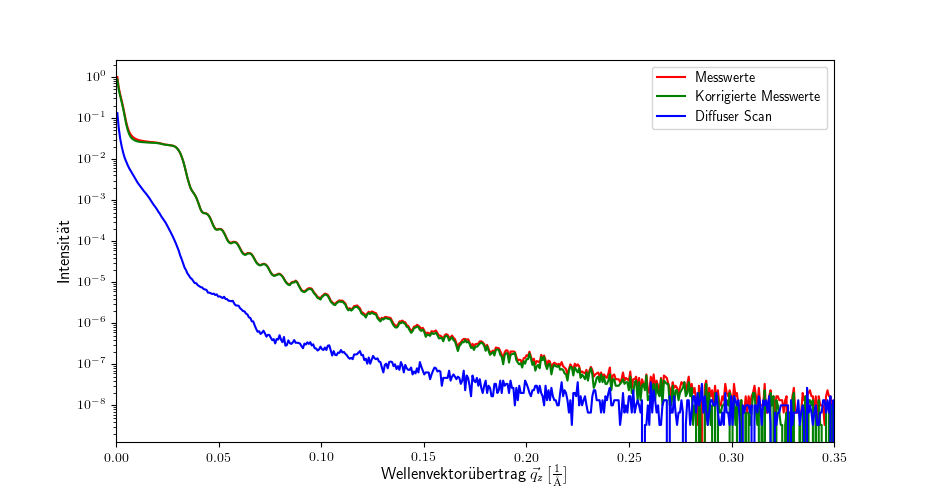
\includegraphics[width=\textwidth]{Berechnung/Plot3.png}
  \caption{Reflektivitätsscan aufgetragen gegen den Wellenvektor.}
  \label{Plot1}
\end{figure}
\subsection{Bestimmung der Probenparameter}
Zur Bestimmung der Probenparameter wird der Parratt-Algorithmus genutzt, um eine Theoriekurve an die  korrigierten Messwerte anzupassen. Die Schichtdicke $d$ lässt sich gemäß \eqref{d} bestimmen, indem die Periodendauer zwischen zwei Maxima vermessen wird. Durch die Lage des kritischen Winkels der Totalreflexion lässt sich danach der Brechungsindex des Substrates bestimmen. Die restlichen Parameter werden solange variiert, bis eine optimale Anpassung an die Messwerte erreicht wird. Hier ergibt sich für die Parameter damit:
\begin{align}
  \text{Brechungsindex Luft}:&\quad n_\text{Luft}=1 \nonumber\\
  \text{Brechungsindex Schicht}:&\quad n_\text{Schicht}= 1-1\cdot10^{-6} \nonumber\\
  \text{Brechungsindex Substrat}:&\quad n_\text{Substrat}=1-6,9\cdot10^{-6} \nonumber\\
  \text{Rauigkeit Schicht}:&\quad \upsigma_\text{Schicht}=15,5\cdot10^{-10} \nonumber\\
  \text{Rauigkeit Substrat}:&\quad \upsigma_\text{Substrat}=9,8\cdot10^{-10} \nonumber\\
  \text{Schichtdicke}:&\quad z=873\,\si{\angstrom}\nonumber
\end{align}
Die Kurve der korrigierten und normierten Messwerte sowie die des Parratt-Algorithmus sind in Abbildung \ref{fit} dargestellt.
\begin{figure}[H]
  \centering
  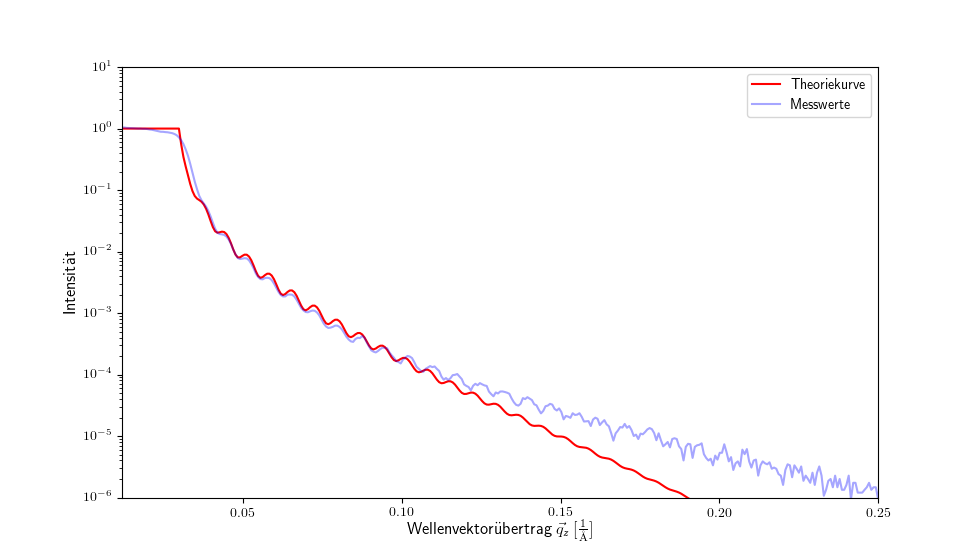
\includegraphics[width=\textwidth]{Berechnung/Fit2.png}
  \caption{Kurve des Parratt-Algorithmus angepasst an die Messwerte.}
  \label{fit}
\end{figure}
